\section{Real-World Evaluation}\label{sec:evaluation}
\noindent We ran three sessions of AtomicOrchid with participants recruited from the local university to trial mixed-initiative coordination in a disaster response scenario. The following sections describe the participants, procedure, session configuration and methods used to collect and analyse quantitative and qualitative data.

\subsection{Participants and procedure}
\noindent  A total of 24 participants (7 of them were female) were recruited through posters and emails, and reimbursed with \pounds 15  for 1.5-2 hours of study. The majority were students of the local university. The procedure consisted of 30 minutes of game play, and about 1 hour of pre-game briefing, consent forms, and a short training session, and a post-game group discussion. 

%Upon arrival in the HQ (set up in a meeting room at the local university), participants were briefed and asked to consent to participate. They were presented with a demographic questionnaire to record gender, occupation, experience of using smartphones and level of map navigation skills.

At the end of the briefing, in which mission objectives and rules were outlined, responder roles were randomly assigned to all participants (fire-fighter, medic, transporter, soldier). HQ was staffed by a different member of the research team in each session in order to mimic an experienced HQ whilst avoiding the same person running HQ every time.  Moreover, responders were provided with a smartphone and HQ coordinators with a laptop. The team was given 5 minutes to discuss a common game strategy. 

%(\textbf{Joel: where did the agent run ? --> Gopal, this should be covered in the previous section I think?})

Field responders were then accompanied to the starting point within the designated game area, about 1 minute walk from headquarters. Once field responders were ready to start, HQ sent a `game start' message. After 30 minutes of game play the field responders returned to the HQ where a group interview was conducted, before participants were debriefed and dismissed.

\subsection{Game sessions}
\noindent We ran one session without the planner agent, and two sessions with the planner agent to be able to compare team performance in the two versions. We also ran a pilot study for each condition to fine tune game configuration. The 8 field responders in each session were randomly allocated a responder so that the whole team had two of each of the four kinds of responder roles. The terrain of the 400x400metres game area includes grassland, a lake, buildings, roads, and footpaths and lawns. There were two safe drop-off zones (i.e., radiation free) and 16 targets in each session. There were four targets for each of the four target types. The target locations, pattern of cloud movement and expansion were kept constant for all game sessions. The pilot study showed that this was a challenging, yet not too overwhelming configuration of game area size, and number of targets to collect in a 30 min game session. 

\subsection{Data collection and analysis}
\noindent We developed a log file replay tool to triangulate video recordings of game action with the timestamped system logs that contain a complete record of the game play, including responders' GPS location, their health status and radioactive exposure, messages, cloud location, locations of target objects and task status.

%Video recordings of field action were catalogued to identify sequences (episodes) of interest (cf. Heath et al., 2010). Key decision points in teaming and task allocation served to index the episodes. Interesting distinct units of interaction were transcribed and triangulated with log files of relevant game activity for deeper analysis. Due to space constraints we can only  present one fragment in this paper to illustrate how human-agent collaboration typically unfolded (TODO).

In order to assess how humans interact with each other and with the agent, we focused on collecting data relevant to agent task allocations and remote messages  that are used to support coordination. In particular, we use speech-act theory (Searle, 1975) to classify messages sent between and among responders and HQ. We focus on the most relevant types of acts in this paper (which are also the most frequently used in AtomicOrchid):

\begin{itemize}
\item Assertives: \textit{speech acts that commit a speaker to the truth of the expressed proposition}; these were a common category as they include messages that contain situational information.
\item Directives: \textit{speech acts that are meant to cause the hearer to take a particular action}, e.g. requests, commands and advice, including task and team allocation messages. 
\end{itemize}
We next detail the results of the trial and then discuss the implications of these results in Section \ref{sec:summary}.

\subsection{Results}
\noindent Overall, 8 targets were rescued in the non-agent condition (Session A), and respectively 12 targets (Session B), and 11 targets (Session C) were rescued in the agent condition. Teams (re-)formed six times in session A, four times in session B and nine times  in session C. Player health after the game was significantly higher (more than twice better) for the agent-assisted sessions (80 for Session B and 82 for Session C) compared to the non-agent assisted session (40/100 in Session A). In fact, one responder `died' in Session A.  

The agent dynamically re-planned 14 times in session B, and 18 times in session C. Most of the times, this was triggered when a target was dropped off in the safe zone (24 times) - as this would free up resources for the algorithm to recompute an allocation - and sometimes this was triggered by a player rejecting the agent's task allocation (8 times) ( as per Section \ref{sec:algo}). 

Finally, Table \ref{tab:msgs} shows the directives (mainly related to task allocation and execution) and assertives (mainly related to situational awareness) sent in the sessions. The next sections draw on how these messages were handled to give a sense of mixed-initiative coordination in the game sessions.

\begin{table}\footnotesize
\begin{tabular}{c | c c | c c c c | c}
 & \multicolumn{2}{c|}{no agent} &  \multicolumn{4}{c|}{agent} & Total \\
 \hline
 Speech acts & \multicolumn{2}{c|}{Session A} & \multicolumn{2}{c}{Session B} & \multicolumn{2}{c|}{Session C} & \\
  & HQ & FR & HQ & FR & HQ & FR & \\
  \hline
  Directives & 89 & 0 & 34 & 2 & 34 & 0 & 159 \\
  Assertives & 33 & 6 & 26 & 16 & 24 & 16 & 121 \\
  \hline
  Total & 122 & 6 & 60 & 18 & 58 & 16 & 280 \\
\end{tabular}
 \label{tab:msgs}
 \caption{Message classification.}
\end{table}


\subsubsection{Handling Task Allocations}
\noindent Fig. \ref{fig:msgs} shows how field responders handled task allocations in the agent and in the non-agent condition. In the non-agent condition, HQ sent 43 task allocation directives. Out of these, the recipient field responders addressed only 15 messages (bringing them up in conversation). Out of these 15, responders chose to ignore the instructions \emph{only once}. The responder ignored the instruction because they were engaged in another task and did not want to abandon it. A further 4 HQ instructions were consistent with a decision to rescue a certain target that has already been made locally by the responders. In 10 cases field responders chose to follow the instructions. Although players were willing to follow HQ's instructions, they failed to correctly follow the instructions due to confusion and misunderstanding in the communication. In fact, only 2 instances of directives from the HQ led to task completion.The field responders accomplished task allocation of the other 6 saved targets locally without being instructed by HQ.

In contrast, when task allocation was handled by the agent, responders accepted 24 tasks, out of which they completed 15 tasks successfully. Even if there was no response or consensus between the responders (in 17 cases), still six out of 17 tasks were completed successfully. In total, 20 task allocations were overridden by a the agent with a new task allocation. 

\begin{figure}[htbp]
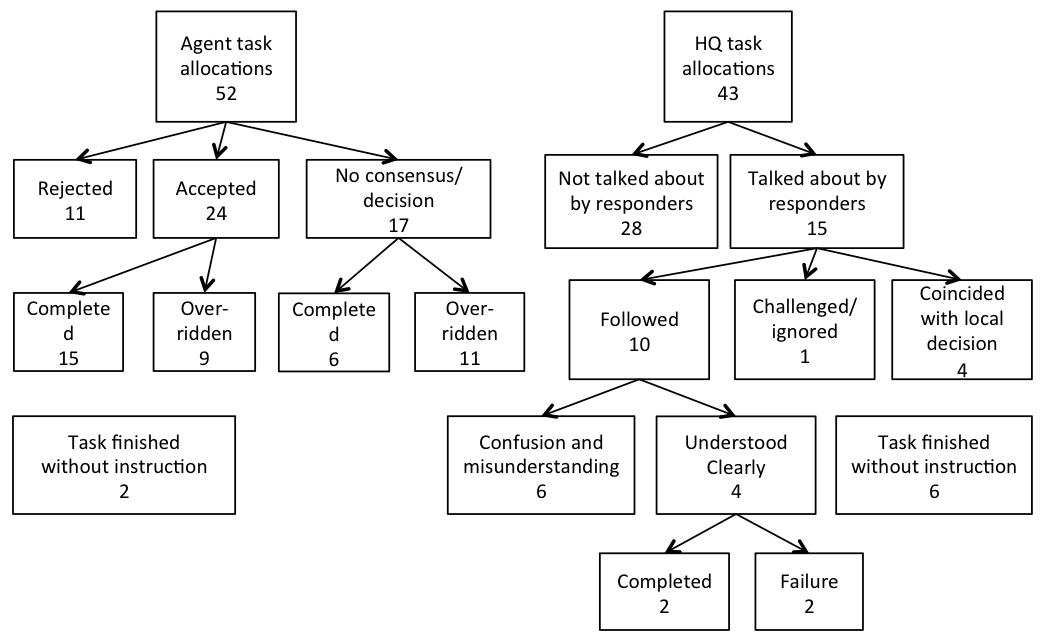
\includegraphics[width=\columnwidth]{message_handling.png}
\label{fig:msgs}
\caption{How task allocations were handled by field responders in the agent version (left) and in the non-agent version (right).}
\end{figure}

\paragraph{Rejecting task allocations}

Field responders rejected the agent's task allocation 11 times in the agent version. All of the rejections happened when the task allocation would have \emph{split existing teams}, or instructed responders to team up with \emph{physically more distant responders}. In most cases (9 out of 11), the rejection triggered re-planning and \emph{adjusted the task allocation} to become consistent with the responder's current team. In the other 2 cases, rejected the task allocation one more time to receive the desired task allocation. 

Overall, players were more likely to reject plan if their proposed teammates were far away from them. For accepted instructions, the average distance between suggested teammates was 12 metres. For rejected instructions, the average distance between suggested teammates was 86 metres.

\subsubsection{The Role of the HQ Commander}
\noindent The burden of task allocation was borne by the HQ commander in the non-agent assisted setting. Instead, in the agent-assisted setting, the HQ commander frequently monitored the allocation of tasks  returned by the agent (57 clicks on `show task' in UI responder status widget). Whereas 43 directives in the non-agent session were task allocations, only 16 out of 68 directives were directly related to task allocations in the agent version. Out of these, HQ reinforced the agent instruction 6 times (e.g., ``SS and LT retrieve 09''), and complemented the agent's task allocation 5 times (``DP and SS, as soon as you can head to 20 before the radiation cloud gets there first''). HQ did `override' the agent instruction in 5 cases.  

In the agent version, the majority of HQ's directives (52 out of 68) and assertives (49 out of 51) focussed on providing situational awareness and safely routing the responders to avoid exposing them to radiation. For example, ``Nk and JL approach drop off 6 by navigating via 10 and 09.'', or ``Radiation cloud is at the east of the National College''. 

\subsubsection{Summary}\label{sec:summary}
The results suggest three key observations with regard to mixed-initiative coordination in the trial:

\begin{itemize}
\item Field responders performed better (rescued more targets), and maintained higher health levels when supported by the agent.
\item Rejecting tasks was a frequently employed method to to trigger re-planning to obtain new task allocations aligned with responder preferences.
\item When task allocation was handled by the agent, the human HQ could focus on providing vital situational awareness to safely route field responders around danger zones; thus demonstrating division of labour and complementary collaboration between human and agent.
\end{itemize}
